\section{Physikalisches Pendel}
Das physikalische Pendel ist wie das Rotationspendel ein einfach harmonisches 
Schwingungssystem. Wie zuvor wird hier die Differentialgelichung mittels der
Momente aufgestellt. 
\[ \boxed{\vec{M}_{\Sigma} 
	= \vec{M}_k + \vec{M}_g	
	= I_z \cdot \ddot{\theta} + d \cdot m \cdot g \cdot \sin(\theta) = 0
} \]
Für kleine Winkel $\theta$ kann $\sin(\theta)$ mit $\theta$ approxmiert
werden.
\[ \boxed{ \sin(\theta) \approx \theta \quad\text{falls }\theta\text{ klein}
} \]
Mit dieser Approximation lässt sich die Differentialgleichung vereinfachen 
zu 
\[ \boxed{M 
	= I_z \cdot \ddot{\theta} + d \cdot m \cdot g \cdot \theta 
	= 0
} \]

\begin{figure}[h!]
	\centering
	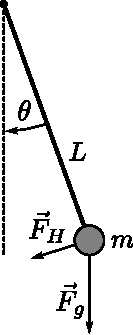
\includegraphics[scale=0.75]{../fig/physikalisches-pendel.pdf}
	\caption{Physikalisches Pendel}
	\label{fig:physikalisches-pendel}
\end{figure}

Das Verhalten ist analog zu den anderen einfach harmonischen 
Schwingungssystemen.
\[ \boxed{\kappa = d \cdot m \cdot g} \qquad 
\text{Schwerpunkt über Drehachse $\Rightarrow$ $\kappa$ negativ} \]
\[ \boxed{\kappa_{tot} = \kappa_1 + \kappa_2 \dots} \]
\[ \boxed{\kappa_{tot} = \sum_{1}^{n} \left(d_n \cdot m_n \cdot g\right) } \]
\[ \boxed{\omega = \sqrt{\frac{\kappa}{I_z}} 
= \sqrt{\frac{m \cdot g \cdot d}{I_z}}} \]
\[ \boxed{f = \frac{\sqrt{\frac{\kappa}{I_z}}}{2 \pi}
= \frac{\sqrt{\frac{m \cdot g \cdot d}{I_z}}}{2 \pi}} \]
\[ \boxed{T = 2 \cdot \pi \cdot \sqrt{\frac{I_z}{m \cdot g \cdot d}}} \]

\subsection{Fadenpendel}
Ein Spezialfall des pysikalischen Pendels ist das sog. Fadenpendel. 
Dies ist ein Pendel, welches einen Massepunkt am Ende eines masselosen
Seils hat. Das Trägheitsmoment bildet sich somit aus einem rein 
steiner'schen Anteil (siehe \textit{Satz von Steiner}, 
Seite \pageref{sec:steiner}).
\[ \boxed{I = m \cdot L^2} \]
Das Verhalten des Systems ist analog zum allgemeinen physikalischen
Pendel. Die Formel sind lediglich vereinfacht durch das spezielle
Trägheitsmoment.
\[ \boxed{\kappa = m \cdot g \cdot L} \]
\[ \boxed{\omega = \sqrt{\frac{g}{L}}} \]
\[ \boxed{f = \frac{\sqrt{\frac{g}{L}}}{2 \cdot \pi}} \]
\[ \boxed{T = 2 \cdot \pi \cdot \sqrt{\frac{L}{g}}} \]
Die Kraft im Seil setzt sich zusammen aus den Radialanteilen der
wirkenden Kräfte.
\[ \boxed{\vec{F}_s 
	= \underbrace{ 
		m \cdot g \cdot \cos(\theta)
	}_{\substack{\text{Radialanteil}\\\text{Gewichtskraft}}}
	+ \underbrace{
		m \cdot \frac{v^2}{L}
	}_{\substack{\text{Radialanteil}\\\text{Rotation}}}
	= m \cdot g \cdot \cos(\theta) + m \cdot \omega^2 \cdot L
} \]

